\documentclass[UTF8]{article}

\usepackage{amsmath}
\usepackage{cases}
\usepackage{cite}
\usepackage{graphicx}
\usepackage[margin=1in]{geometry}
\geometry{a4paper}
\usepackage{fancyhdr}
\pagestyle{fancy}
\fancyhf{}
\usepackage{float}  %设置图片浮动位置的宏包
\usepackage{subfigure}

\usepackage{caption}
\usepackage{booktabs}

\title{Study of the polarisation properties of light}
\author{by 22 Artificial Intelligence ChenxuZhang}
\date{2023.3.16}
\pagenumbering{arabic}

\begin{document}
	
	\fancyhead[L]{ChenxuZhang}
	\fancyhead[C]{Study of the polarisation properties of light}
	\fancyhead[R]{ID 202264691028}
	\fancyfoot[C]{\thepage}
	
	\maketitle
	\tableofcontents
	\newpage
	
	\section{Abstract}
	In 1811, the French physicist D.F.J. Arago, while studying the birefringence of quartz crystals, discovered that when a ray of polarised light propagates along the direction of the quartz crystal's optical axis, its plane of vibration turns at an angle with respect to the original direction, a phenomenon known as spin. Subsequently, physicists such as Biot discovered that some vapours and liquids, such as sodium chlorate solutions, sugar solutions, turpentine and many organic compounds, all exhibit this phenomenon. The phenomenon of the spin of substances has a wide range of applications in various fields, such as in the pharmaceutical industry, drug testing and commodity testing departments commonly used to determine the content of certain substances in some drugs and commodities (such as vitamin C in multivitamins, nicotine in cigarettes, camphor in mothballs, etc.), the sugar industry to determine the concentration of sugar, etc. It is important to study the relationship between the spinability of a solution and its concentration and to learn how to use the spinability of a substance to measure its spin rate and concentration. The focus of this paper is to verify Marius' law and to determine the spin rate of a 15\% glucose solution and to investigate the factors influencing the spin rate of a sample solution.\\
	\textbf{Result:}the real experimental results are similar to the theoretical equation, $I\sim \cos ^{2} \alpha $ is proportional within the error allowed, verifying Marius' law.The average angular difference between the five experiments was $11 ^{\circ} {43}'{2}''$, resulting in $48.614\pm 0.869\left ( ^{\circ} \cdot cm^{3} \cdot g^{-1} \cdot dm^{-1} \right )$, which is not too far from the ideal figure of 50$\left ( ^{\circ} \cdot cm^{3} \cdot g^{-1} \cdot dm^{-1} \right )$.A discussion of the factors influencing the spin rate of the sample solutions is included in the Data Analysis and Experimental Procedures section.\\
	\\
	\textbf{Key Words: Marius' Law,15\% dextrose solution,Difference-by-difference, least squares, spin rate}
	
	
	\section{Purpose of the experiment}

       a.Learn to assemble and use a spinograph.\\
     b.Deepen our understanding of the polarisation of light and the spinning nature of matter.\\
       c.Knowledge of methods for determining the spin rate and concentration of glucose solutions.
	
	

	
	
	\section{Experimental apparatus}
	
		\subsection{OEX-PSP polarised light spin tester}
	 The complete set includes a semiconductor laser, guide rail, polariser with turntable, light intensity detector, sample tube holder and adjustment device.As shown in Fig. 1
	\begin{figure}[H]
	    \begin{minipage}[t]{0.5\linewidth}
	    	\centering
	    	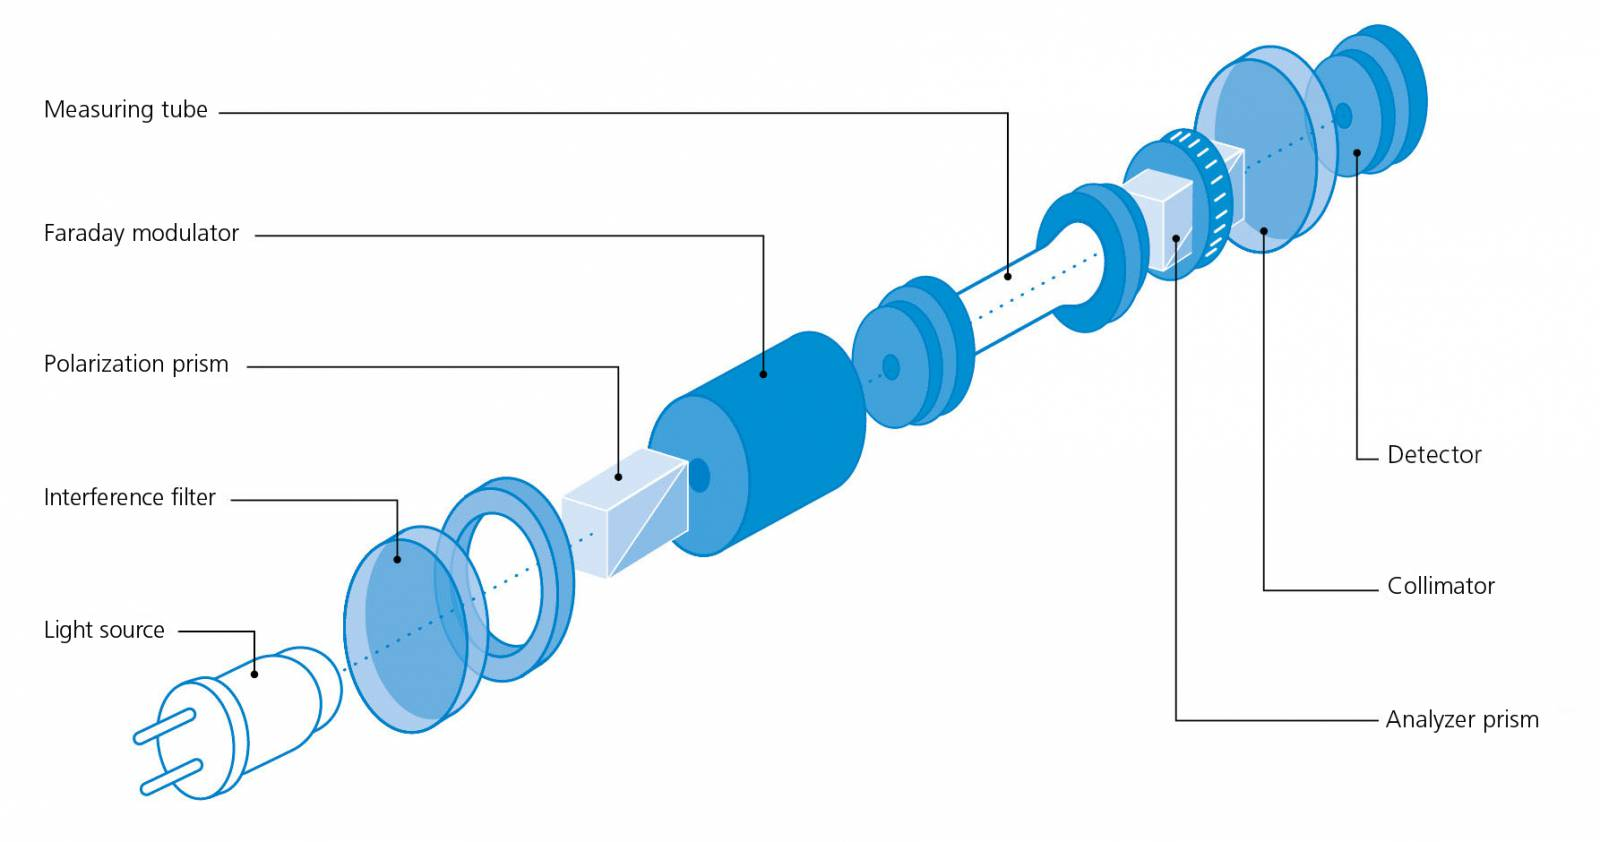
\includegraphics[clip,scale=0.1]{figure/fig1.jpg}
	    	\caption{OEX-PSP polarised light spin tester}
	    	\label{figure.1}
	    \end{minipage}
        \begin{minipage}[t]{0.5\linewidth}
        	\centering
        	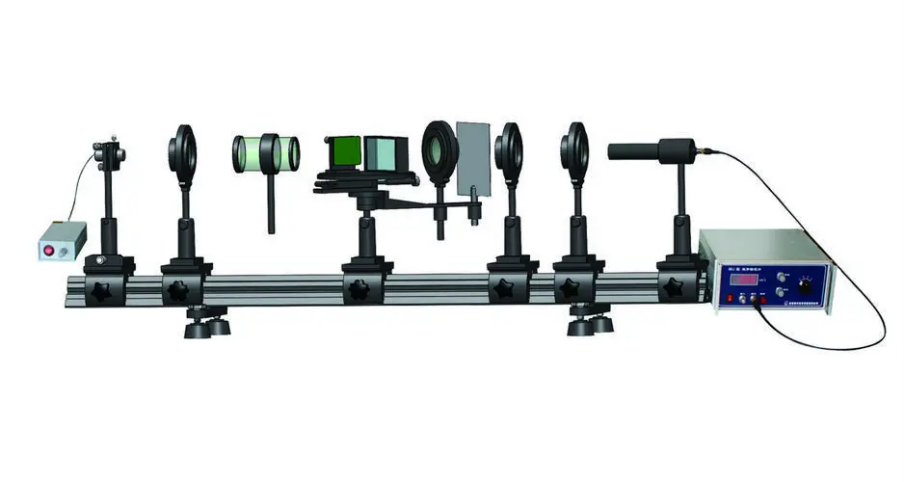
\includegraphics[clip,scale=0.8,trim={0 30 0 0}]{figure/fig2.png}
        	\caption{Physical demonstration drawings}
        	\label{figure.2}
        \end{minipage}
		\end{figure}
	\subsection{Sample tube }
	Sample tube with 15\% mass concentration of glucose solution.Located between the deflector and the detector, it is used to deflect the laser for the purpose of detecting the spin rate. It is also necessary to ensure that the sample tube is at the same height and level as the front and rear mirrors during use.
	  \begin{figure}[H]
	  	\centering
	  	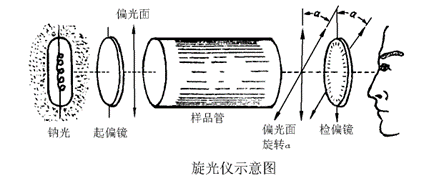
\includegraphics[clip,scale=1,trim={0 22 0 0}]{figure/fig3.png}
	  	\caption{Detailed explanation of each part of the experimental apparatus}
	  	\label{figure.3}
	  \end{figure}
	
	
	
	

	
	\section{Experimental principles}
	Many organic compounds, such as petroleum and glucose, have spin properties due to the asymmetry of their molecular structure. Spin is present in all states of these substances, including solutions of these substances. Some minerals (e.g. quartz, jusha, etc.) also have spinodal properties, which are due to their crystalline structure, so that when the crystalline form disappears, the spinodal properties also disappear.
	
	
	\subsection{Polarizability of light}
	Light is an electromagnetic wave, and since the action of electromagnetic waves on matter is mainly the electric field, the electric field strength E is referred to in optics as the light vector. In a plane perpendicular to the direction of propagation of the light wave, the light vector may have different directions of vibration, and the state in which the light vector remains in a certain direction of vibration is usually referred to as the polarisation state. If the light in the process of propagation, if the light vector to maintain a fixed plane vibration, this vibration state is called plane vibration state, this plane is called vibration surface (see Figure 4). At this time the light vector in the plane perpendicular to the direction of propagation and the projection of a straight line, so also known as the line polarization state. If the light vector rotates around the direction of propagation, its endpoint depicts the orbit of a circle, this polarization state is called circular polarization state. If the endpoint of the light vector rotates in an ellipse, it becomes an elliptical polarization state.(see Figure 5)
		\begin{figure}[H]
		\begin{minipage}[t]{0.5\linewidth}
			\centering
			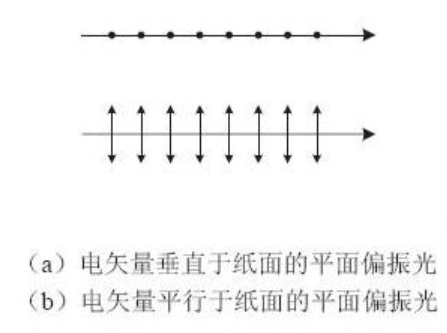
\includegraphics[clip,scale=1,trim={0 60 0 0}]{figure/fig4.png}
			\caption{Planar polarised light}
			\label{figure.4}
		\end{minipage}
		\begin{minipage}[t]{0.5\linewidth}
			\centering
			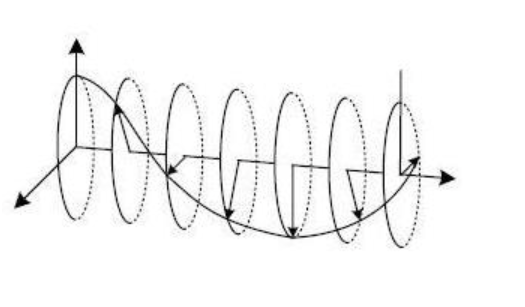
\includegraphics[clip,scale=0.8]{figure/fig5.png}
			\caption{Elliptically polarised light}
			\label{figure.5}
		\end{minipage}
	\end{figure}

	
	\subsection{Polarizer}
	Although ordinary light sources emit natural light, there are various kinds of polarised light in nature. The widely used device for polarised light is the artificial polariser, which uses dichroism to obtain polarised light (some isotropic media, under some kind of action, will show anisotropy and can strongly absorb the component of the incident light vector in a certain direction and pass its vertical component, thus changing the incident natural light into polarised light media of this (This property is called dichroism.). . Polarising devices can be used to change natural light into plane polarised light - polarisation, or to identify linearly polarised light, natural light and partially polarised light - polarisation detection. The polarizer used for polarization is called a polarizer, and the polarization device used for polarization detection is called a polarization detector. In fact, the polariser and the detector are universal.
	\subsection{Marius' Law}
	\subsubsection{about Marius' Law}
	Malus’ law states that the intensity of plane-polarized light that passes through an analyzer varies as the square of the cosine of the angle between the plane of the polarizer and the transmission axes of the analyzer.

	\begin{figure}[H]
	\begin{minipage}[t]{0.5\linewidth}
		\centering
		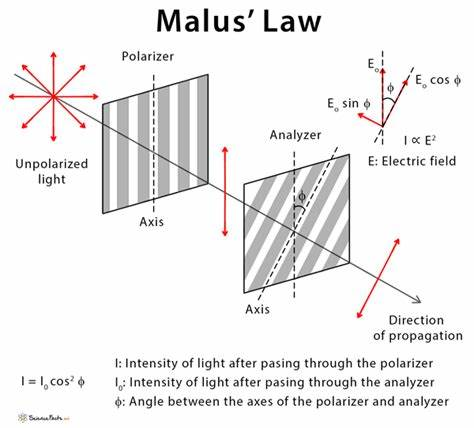
\includegraphics[clip,scale=0.31,trim={0 73 0 0}]{figure/fig6.jpg}
	\end{minipage}
	\begin{minipage}[t]{0.5\linewidth}
		\centering
		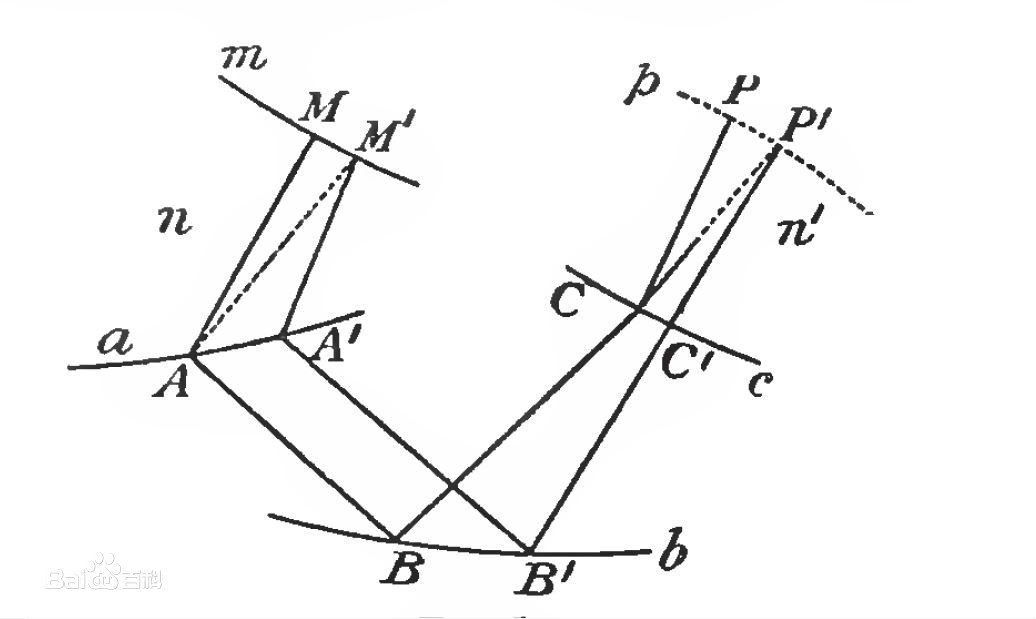
\includegraphics[clip,scale=0.18]{figure/fig7.jpg}
	\end{minipage}
\caption{Schematic representation of the principle of Marius' Law}
\label{figure.6}
\end{figure}
	
	\subsubsection{Formula derivation}
	The angle between the transmission directions of the two polarizers is $\alpha$. The amplitude of the polarized light through the polarizer is $A_{0}$, and the amplitude through the polarizer is A. Then we have:
   \begin{eqnarray}
        A=A_{0} \cos \alpha 
   \end{eqnarray}

	Because the detector detects the light intensity, the light intensity I is:
	\begin{eqnarray}
	I=A^{2} 
	\end{eqnarray}

	 Continuing the derivation yields:
	\begin{eqnarray}
		I=\left (A_{0}\cos {\alpha }   \right ) ^{2} =I_{0} \cos ^{2} \alpha 
	\end{eqnarray}

    \subsection{Rotation rate}
    \subsubsection{About spin rate $\varphi $ }
    When polarised light passes through these substances, the vibrating surface is rotated by an angle $\varphi $ in the direction of light propagation, a phenomenon known as spin.
    
    \textbf{Research shows that:}
    
    a.For a solid substance with rotational properties, when polarized light passes through it, the angle of rotation $\varphi $ of the polarization plane is proportional to the thickness $l$ of thel light passing through the solid substance, i.e.\\
    	\begin{eqnarray}
    	\varphi =\alpha l 
        \end{eqnarray}
    
    b.For liquids with rotational properties, when polarised light passes through it, the angle of rotation of the polarisation plane $\varphi $ is proportional to the thickness $l$ of the light passing through the solution and the concentration $c$ of the solution, i.e.
    \begin{eqnarray}
    \varphi =\alpha lc
    \end{eqnarray}

	The $\varphi $ is called the rotational index of a substance and is related to the wavelength of the incident light wave and the rotating substance. The angle of rotation of the vibrational plane of a substance is different for different wavelengths of linearly polarised light passing through a certain length of rotating material, a phenomenon known as rotational dispersion. $\varphi $ is also temperature dependent, but not by much. For most substances, the spin rate decreases by a few thousandths of a degree for every $1^\circ C$ increase in temperature.
	\subsubsection{About levorotatory}
	There are left- and right-spinning substances. When the experimenter looks into the light, substances whose vibrating surface rotates clockwise are called right-handed substances and vice versa for left-handed substances.
	  \begin{figure}[H]
		\centering
		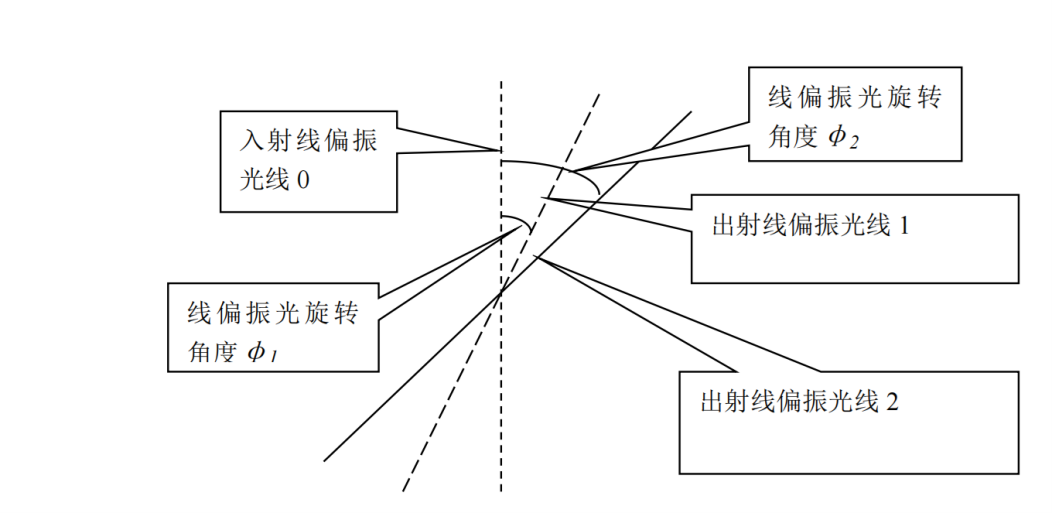
\includegraphics[clip,scale=0.5,trim={30 0 0 20}]{figure/fig8.png}
		\caption{Diagram of right-hand rotation}
		\label{figure.7}
	\end{figure}

	As shown above: a simple way to determine this is to still choose $l_{1} $ and $l_{2} $ as prime numbers, $l_{1} > l_{2} $ and the difference 
	is not large; if $\theta _{2} > \theta _{1} $ is measured, the substance can be judged to be a right-handed light substance and vice versa.
	
	\section{Contents and Steps}
	
	\subsection{Determining the polarizability of a light source and verifying Marius' law}
    A.Place the laser and the light intensity detector on the rail, then turn on the light intensity detector power switch and, when there are no other components on the rail, cause the laser to be directed vertically into the light intensity detector.
    \\
    \\B.Place the deflector, adjust the height of the deflector so that the laser passes through its centre; adjust the angle of the deflector so that the light intensity reading is maximum, start from the maximum light intensity position to the rotation of $90^\circ$, change the angle of the deflector one by one, record a set of data every $15^\circ$, and determine the polarization state of the light source according to the data obtained.
     \begin{figure}[h]
    	\centering
    	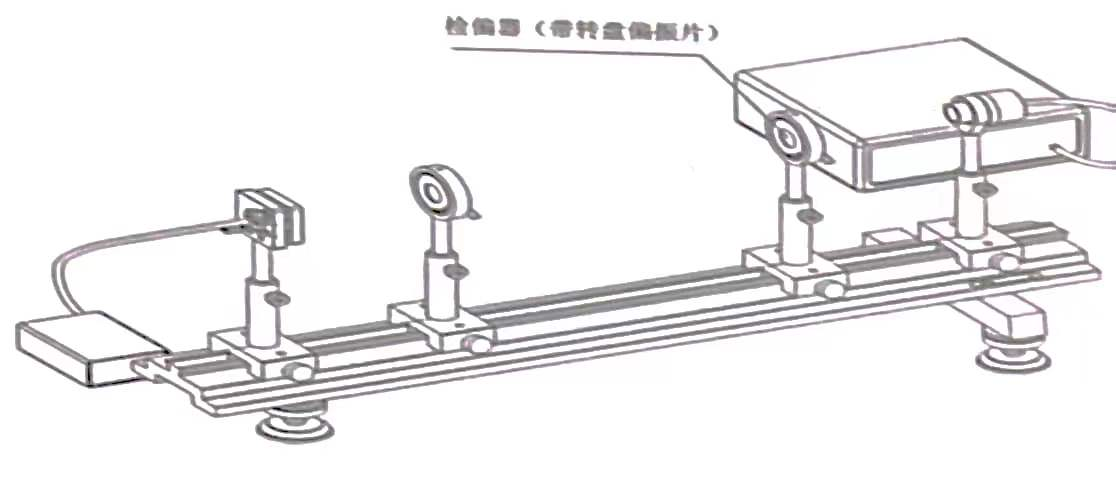
\includegraphics[clip,scale=0.2,trim={0 0 0 0}]{figure/fig9.jpg}
    	\caption{Operation demonstration diagram}
    	\label{figure.8}
    \end{figure}
   \\C.If it is concluded that the light source is linearly polarized light, use these data to make a graph of $I\sim \left ( \cos \theta  \right ) ^{2} $ to verify Marius' law.
    \\
    \\D.If the light source is not linearly polarised, set the polariser back to the position where the light intensity reading is maximum, put in the detector and adjust the detector so that the light intensity reading is maximum, starting from this position and rotating it by $90^\circ$, change the angle of the detector one at a time and record a set of data every $15^\circ$. Finally, the data obtained is used to verify Marius' law.
	
	\subsection{Measurement of the spin rate and concentration of glucose solutions using a polarised light spin tester}
	\subsubsection{Assembly of polarised light spinners}
	A.The semiconductor laser, deflector, sample tube holder and light intensity detector are mounted and fixed to the optical tool holder and the coaxial contour is adjusted so that the laser emits a laser that passes vertically through the centre of the deflector and light intensity detector.
	\\
	\\B.Adjust the polarizer dial so that the polarized light output is the strongest, and fix the polarizer on the slide of the guide so that the polarizer and the polarizer are parallel and coaxial at the same height. Adjust the polarizer dial so that the light output from the polarizer is the strongest and the direction of polarization of the polarizer is perpendicular to the direction of polarization of the starter, and note the angle value ${\theta  }'   $ of $P_{2} $ at this point. Rotate $P_{2} $ by $360^\circ$ and observe the change in light intensity during the rotation.
	 \begin{figure}[H]
		\centering
		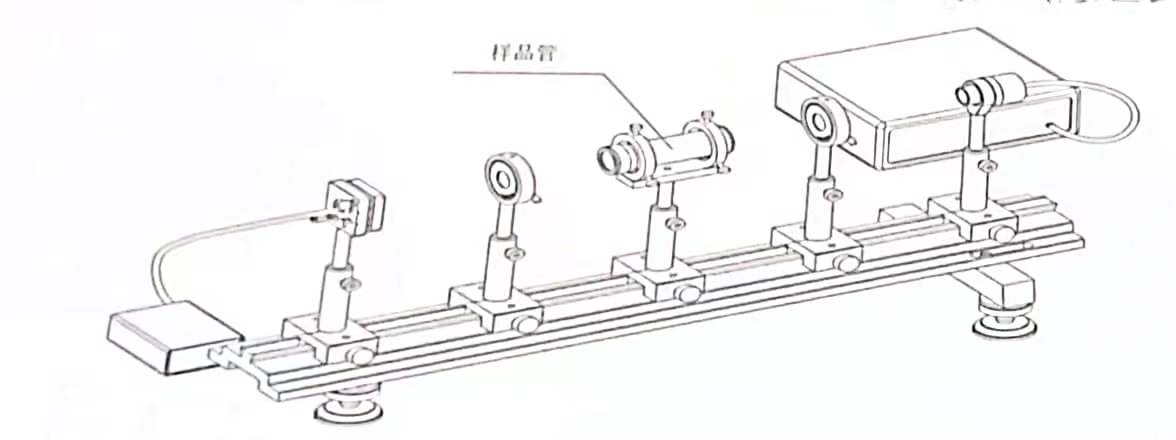
\includegraphics[clip,scale=0.2,trim={0 0 0 10}]{figure/fig10.jpg}
		\caption{Operation demonstration diagram}
		\label{figure.9}
	\end{figure}
	
	\subsubsection{Measurement of the spin rate of glucose solutions}
	A.Place the sample tube with pure water on the holder and use a piece of white paper to observe whether the light point incident to the sample tube and the light point out of the sample tube are of the same shape to check whether the glass sample tube is coaxial with the laser beam at the same height. If they are not coaxial, adjust the adjustment screw under the sample tube holder to achieve coaxiality.
	\\
	\\B.Observe the spin phenomenon in pure water. Adjust the detector dial to minimise the output light intensity, note the angular value of $P_{2} $ at this point $\theta _{0} $ and compare $\theta _{0} $ with ${\theta  }'   $. After taking one reading of the angle of $\theta _{0} $, rotate $P_{2} $ $360^\circ$ degrees in one direction and take another reading, 5 times in total.
	\\
	\\C.A sample tube filled with a 15\% mass concentration of glucose solution is placed on the sample tube holder. At this point it can be observed that the light intensity through the detector is not the minimum value, but must be rotated to a certain $\theta _{i} $ angle before the light intensity detector shows the minimum value, from which the angle $\theta _{i} $ corresponding to  $P_{2} $ when the sample is a glucose solution is measured (5 times in total). The difference between $\theta _{i} $ and $\theta _{0} $ is the rotational luminosity of the glucose solution.
	\\
	\\D.Use vernier calipers to measure the length of the sample tube L (take 5 tubes and measure each once) and the ambient temperature t (once before, once during and once after the experiment).
	\\
	\\E.Using the difference-by-difference method, find the spin rate of the substance $\left [ \alpha  \right ] _{L}^{t} $ and find the uncertainty of the spin rate.
	\begin{eqnarray} \theta & = & \left [ \alpha  \right ] _{L}^{t} lc \Longleftrightarrow \left [ \alpha  \right ] _{L}^{t}=\frac{\theta }{lc} \end{eqnarray}
	%图一般很大,建议换页。
	\section{Data processing}
	\subsection{Determining the polarisation of a light source with a single starter}
	Place the laser and light intensity detector on the rail, then turn on the light intensity detector power switch and, when there are no other components on the rail, cause the laser to be directed vertically into the light intensity detector. Place the deflector and adjust the height of the deflector so that the laser passes through its centre. Adjust the angle of the deflector to maximise the light intensity reading, starting from the maximum light intensity position and rotating it by $90^\circ$, changing the angle of the deflector one at a time and recording a set of data at $15^\circ$ intervals as follows:
	\begin{center}
			\begin{tabular}{ccc}
				\toprule
				Number & Angle of deflector$\left ( ^{\circ}  \right ) $ & Light intensity$\left ( 10^{-7}A  \right ) $\\
				\midrule
				1st & $160^{\circ} {0}' $ & 6.450 \\
				2ed & $175^{\circ} {0}' $ & 5.630 \\
				3rd & $190^{\circ} {0}' $ & 3.850 \\
				4th & $205^{\circ} {0}' $ & 2.430 \\
				5th & $220^{\circ} {0}' $ & 1.778 \\
				6th & $235^{\circ} {0}' $ & 1.950 \\
			    \bottomrule
				\end{tabular}
		\end{center}
	
	Based on the data collected, we plotted scatter plots in a coordinate system, followed by linear regression using least squares to obtain the regression line l. The images are as follows:
	\begin{figure}[H]
		\begin{minipage}[t]{0.5\linewidth}
			\centering
			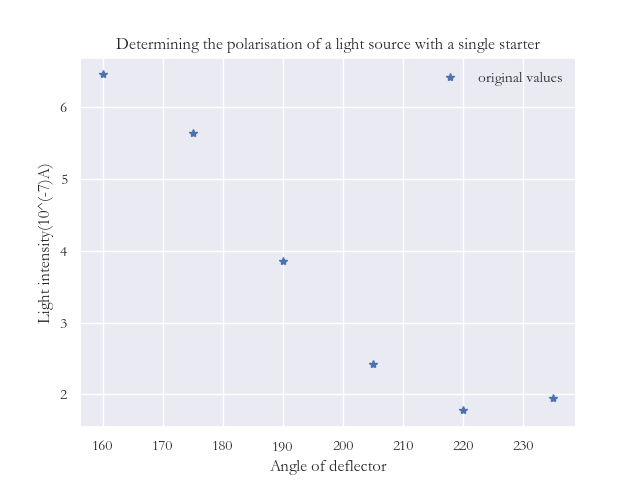
\includegraphics[clip,scale=0.5]{figure/fig12.png}
			\caption{Scatterplot}
			\label{figure.10}
		\end{minipage}
		\begin{minipage}[t]{0.5\linewidth}
			\centering
			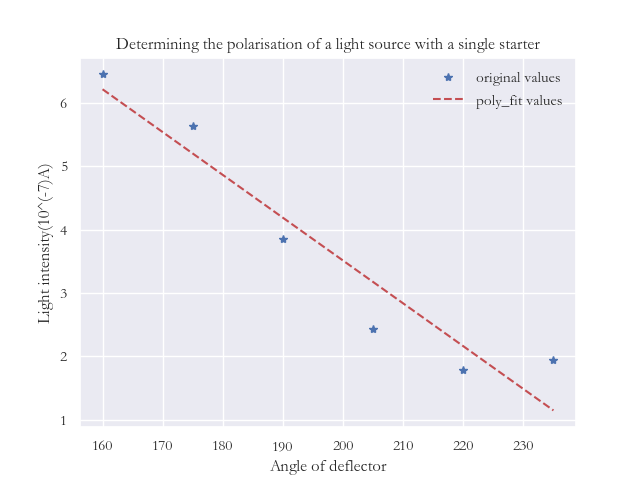
\includegraphics[clip,scale=0.5,trim={0 0 0 0}]{figure/Fig11.png}
			\caption{Least Squares Regression}
			\label{figure.11}
		\end{minipage}
	\end{figure}

    The fitted trend line is obtained by least squares as:
   \begin{eqnarray}y= -0.0676 x + 17.037\left ( R^{2}= 0.9137 \right ) \end{eqnarray}
    
    The correlation coefficient was observed to be small, so the experimental data may be incorrect. Using the Grubbs criterion, taking the significance level $a=0.01 $ and the number of measurements $n = 6$, checking the table gives $ g_{0} \left ( 10,0.01 \right ) =1.94$, so the sixth set of data is anomalous.
    \begin{eqnarray}g_{\sigma } > g_{0} \left ( 10,0.01 \right ) =1.94 \end{eqnarray}
    
    From this, the first experimental data cannot determine whether the light source is linearly polarised, and the error may be due to a systematic error, i.e. a problem with the polariser. Further experiments will be required to confirm this. Here we have excluded the data from the sixth experiment as an outlier and re-plotted it to obtain the following graph(Figure.12) and the following relationship:
     \begin{eqnarray}y= -0.08363 x + 19.9167\left ( R^{2}= 0.9714 \right ) \end{eqnarray}
    \begin{figure}[h]
    	\centering
    	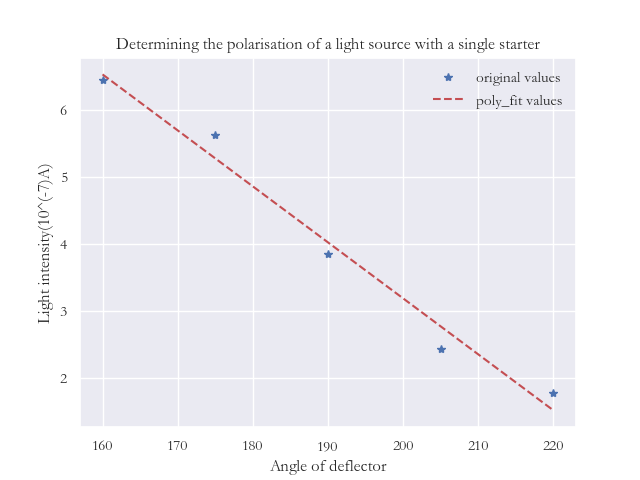
\includegraphics[clip,scale=0.7,trim={0 0 0 0}]{figure/fig13.png}
    	\caption{Regression image after excluding outliers}
    	\label{figure.12}
    \end{figure}

    Ultimately we can conclude that the data after excluding the outliers is essentially in line with the linear variation. Thus, within the limits of error, the polariser does serve the purpose of creating polarised light. However, there are still systematic errors in the experiment, including: some problems with the polariser itself; and changes in ambient light can interfere with the experiment to some extent.
    
    \newpage
    \subsection{Verification of Marius' Law}
    
Based on the experimental procedure described above, we added a bias detector between the deflector and the detector so that it was on a level with the other devices. This is how we begin to verify Marius' law. The deflector is placed and the height of the deflector is adjusted so that the laser passes through its centre. The angle of the deflector is adjusted to the position of maximum light intensity measured in the previous experiment, then the angle of the deflector is kept constant and the deflector is adjusted to the position of maximum light intensity and the angle is recorded at this point. The angle of the deflector is then changed from the maximum light intensity position to a rotation of $90^\circ$, with a set of data recorded at $15^\circ$ intervals, as follows.
	\begin{center}
	\begin{tabular}{ccc}
		\toprule
		Number & Angle of deflector$\left ( ^{\circ}  \right ) $ & Light intensity$\left ( 10^{-7}A  \right ) $\\
		\midrule
		1st & $-18^{\circ} {0}' $ & 6.450 \\
		2ed & $-3^{\circ} {0}' $ & 6.030 \\
		3rd & $12^{\circ} {0}' $ & 3.660 \\
		4th & $27^{\circ} {0}' $ & 3.120 \\
		5th & $42^{\circ} {0}' $ & 1.517 \\
		6th & $57^{\circ} {0}' $ & 0.461 \\
		\bottomrule
	\end{tabular}
\end{center}
	
	We then further processed the data by referring to Marius's law. We kept the light intensity of each test and the maximum light intensity value, and combined this with the square of the cosine of each adjustment angle to make the following table:
	
		\begin{center}
		\begin{tabular}{cccc}
			\toprule
			Number & Max Light intensity$\left ( 10^{-7}A  \right ) $  & Light intensity$\left ( 10^{-7}A  \right ) $& $\cos ^{2}\Delta \theta   $\\
			\midrule
			1st & 6.450 & 6.450 & 1.000\\
			2ed & 6.450 & 6.030 & 0.933\\
			3rd & 6.450 & 3.660 & 0.750\\
			4th & 6.450 & 3.120 & 0.500\\
			5th & 6.450 & 1.517 & 0.250\\
			6th & 6.450 & 0.461 & 0.067\\
			\bottomrule
		\end{tabular}
	\end{center}
	
	Next we made a least squares image of the ratio of 1234 to the light intensity after passing the bias detector and obtained the following equation.
	 \begin{eqnarray}y=  6.4152x -0.08586\left ( R^{2}= 0.9757 \right ) \end{eqnarray}
	
	\begin{figure}[H]
		\begin{minipage}[t]{0.5\linewidth}
			\centering
			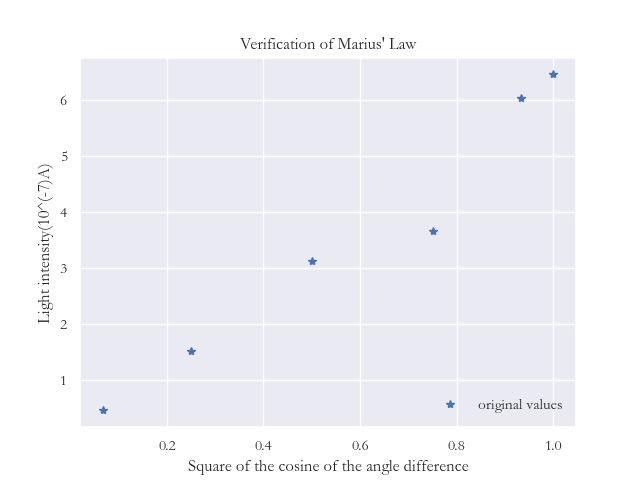
\includegraphics[clip,scale=0.5]{figure/fig14.png}
			\caption{Scatterplot}
			\label{figure.13}
		\end{minipage}
		\begin{minipage}[t]{0.5\linewidth}
			\centering
			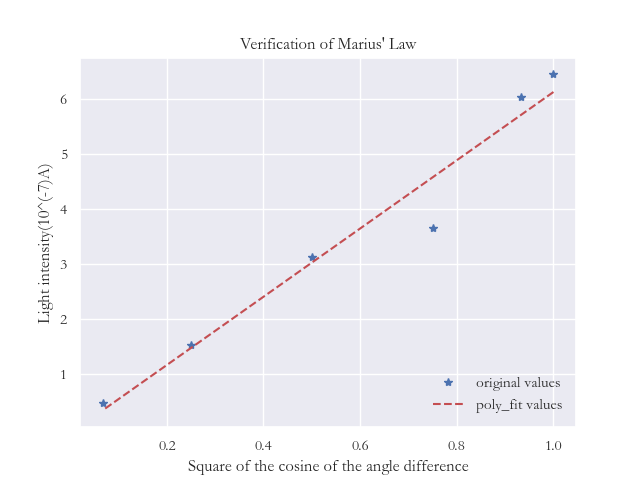
\includegraphics[clip,scale=0.5,trim={0 0 0 0}]{figure/fig15.png}
			\caption{Least Squares Regression}
			\label{figure.14}
		\end{minipage}
	\end{figure}

From the above analysis, we can find that $\cos ^{2}\Delta \theta   $ and light intensity I are roughly proportional, within the error allowed, and the proportionality equation can be approximated as:
\begin{eqnarray}y=  6.4152x -0.08586 \Rightarrow y =6.42x \end{eqnarray}
\begin{eqnarray}\frac{I}{\cos ^{2}\Delta \theta  } =\frac{y}{x}=6.42\approx 6.45 = I_{0} \end{eqnarray}

Therefore, we can find that the experimental data satisfy Marius's law within the margin of error.
\begin{eqnarray}
	I=I_{0} \cos ^{2} \alpha 
\end{eqnarray}

The data from this experiment are still somewhat inaccurate from the actual findings, mainly guessed to be systematic errors, stemming from the instability of the ambient light, and the presence of measurement errors in some of the data. Further research is needed for subsequent experiments.

\subsection{Spin photometry of 15\% glucose solution}
After the above experiments, we kept the original equipment intact, added two holders between the bias starter and the bias detector and prepared sample tubes filled with 15\% glucose solution. The length of the sample tube of glucose solution was first measured. We took several measurements of it using a scale and recorded the results as follows:
	\begin{center}
	\begin{tabular}{cc}
		\toprule
		Number & Measurement results $\left ( dm \right ) $\\
		\midrule
		1st & 1.596 \\
		2ed & 1.621 \\
		3rd & 1.603 \\
		4th & 1.612\\
		5th & 1.610\\
		6th & 1.611 \\
		\bottomrule
	\end{tabular}
\end{center}

Using the averaging formula, we can calculate the average of the sample tubes obtained from six measurements:
\begin{eqnarray}
	\bar{L}  =  \frac{\sum_{i=1}^{6} L_{i} }{6}  =  1.609 \left ( dm \right )  
\end{eqnarray}
\begin{eqnarray}
	\sigma _{L} =  \sqrt{\frac{\sum_{i = 1}^{6} \Delta L_{i } ^{2}}{6-1} }  = 0.00852\left ( dm \right ) 
\end{eqnarray}

Again, judged by the Grubbs criterion, all data is in accordance with the requirements.
\begin{eqnarray}
	\bar{L}  =  1.610\pm 0.009\left ( dm \right )   
\end{eqnarray}




The sample tube is placed on the stand and the height is adjusted to a situation where each device is at equal height. The sample tube is then removed and the deflector is adjusted to the maximum light intensity, then the deflector is adjusted so that the minimum light intensity is received at this point. The angle of the detector at this point was recorded as $\theta _{0} $, satisfying:
\begin{eqnarray}\theta _{0} = 70^{\circ}{56}'  \qquad  I_{0}=0.222\left ( 10^{-7} A \right )  \end{eqnarray}

Next, place the sample tube. The detector is readjusted to minimise the light intensity received and the light intensity and detector angle are recorded at this point. The detector is then rotated 360 degrees and the sample tube is adjusted. The above steps are repeated several times and the data is recorded as shown in the table below. After repeating the experiment five times, we subtracted the recorded data from the initial data to obtain $\Delta \theta \quad \Delta I$, which was eventually collated into the following table:
	\begin{center}
	\begin{tabular}{ccccc}
		\toprule
		Number & $\theta _{i} $ & $L _{i} $ & $\Delta \theta $ & $\Delta I$\\
		\midrule
		1st & $60^{\circ} {0}' $ & 0.200 & $10^{\circ} {56}' $ & 0.022\\
		2ed & $58^{\circ} {44}' $ & 0.204 & $12^{\circ} {12}' $ & 0.018\\
		3rd & $58^{\circ} {36}' $ & 0.202 & $12^{\circ} {20}' $ & 0.020\\
		4th & $59^{\circ} {24}' $ & 0.198 & $11^{\circ} {32}' $ & 0.024\\
		5th & $59^{\circ} {20}' $ & 0.197 & $11^{\circ} {36}' $ & 0.025\\
		\bottomrule
	\end{tabular}
\end{center}

Based on the difference-by-difference method, we were able to use the experimental data to calculate the mean rotational luminosity of the sample solution $\Delta \bar{\theta } $:
\begin{eqnarray}\Delta \bar{\theta } =\frac{\sum \Delta \theta _{i} }{5} =11 ^{\circ} {43}'{2}'' \end{eqnarray}

Finally brought into the equation for the spin power, we can finally obtain the spin power of the 15\% glucose solution as:   $ \left ( ^{\circ} \cdot cm^{3} \cdot g^{-1} \cdot dm^{-1} \right ) $
\begin{eqnarray}\left [ \alpha  \right ] _{L}^{t}=\frac{\theta }{lc}=\frac{\Delta \bar{\theta } }{\bar{L}c } =\frac{11.733^{\circ} }{1.609\times 0.15}=48.614\pm 0.869   \end{eqnarray}

A review of the information shows that a 15\% glucose solution has a spin rate of about 50. Therefore, the data obtained from the experimental calculations are basically close. The sources of error are mainly systematic errors, which are manifested in the unstable ambient light affecting the measurement of the data, the small number of samples, the existence of certain errors in the measurement, and the imprecise measurement of the experimental equipment. Further experimental studies need to be awaited.


\section{Conclusion and analysis}
\subsection{Experimental conclusion}
A.From the results of the experiment, the results were realistic and generally close to the real results, and the experiment was more successful.\\
\\
B.Marius' law verification: the real experimental results are similar to the theoretical equation, $I\sim \cos ^{2} \alpha $ is proportional within the error allowed, verifying Marius' law.\\
\\
C.The average angular difference between the five experiments was $11 ^{\circ} {43}'{2}''$, resulting in $48.614\pm 0.869\left ( ^{\circ} \cdot cm^{3} \cdot g^{-1} \cdot dm^{-1} \right )$, which is not too far from the ideal figure of 50$\left ( ^{\circ} \cdot cm^{3} \cdot g^{-1} \cdot dm^{-1} \right )$.


\subsection{Experimental error analysis}
A.photocurrent meter error: experiments, photocurrent meter readings are unstable, causing difficulties in reading.\\
\\
B.Device error: The deflector and deflector cannot form a perfectly parallel relationship with each other, resulting in a certain error in the measurement.\\
\\
C.Ambient light error: the presence of natural light intensity causes deviations between the instrument indication and the actual laser generated light intensity\\
\\
D.Equipment problems lead to incorrect results: During experiments using a polariser to check for the presence of polarised light, we found that there were intervals where the light intensity received by the receiver did not change, no matter how the angle of the polariser was adjusted. This made it impossible to accurately find the angle at which the light intensity was at its maximum, causing problems in the calculation of the data and leading to the conclusion that the light was polarised in some of the intervals. Further experiments are needed to determine the exact problem.

	
\end{document}  